\section{Colors and Light}
\greenbf{CIE Experiment:} subject is shown two stimuli at the same time, one with the pure spectral color, the other a linear combination of the three primaries (RGB). Subject can control how much primaries were dimmed and asked to match the second stimulus to the first. $\rightarrow$ find how humans perceive color. Can also add red light to reference if impossible to match $\rightarrow$ negative red values. \\
\greenbf{xyY color space:} x,y control chormacity, Y is luminance. 
\begin{wrapfigure}[9]{l}{0.4\columnwidth} %changing the dimensions will mess everything up so be careful!!
    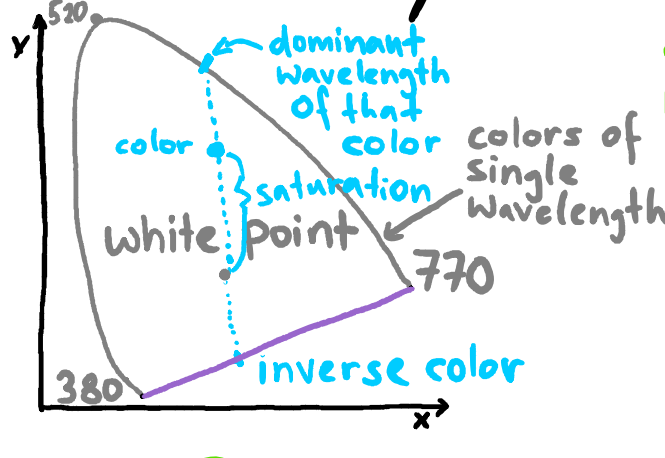
\includegraphics[width=0.4\columnwidth]{arjun/cie-chromacity.png}
\end{wrapfigure}
\greenbf{White point:} $(x,y) = (0.3,0.3)$ \\
\greenbf{Purple line:} Line connecting 380 and 770mm of non-spectral colors. \\
\greenbf{Isoline:}  a line with about constant distance to the border \\
\greenbf{Inverse color:} Intersection of line drawn by the color and white point with the opposite border. 
\greenbf{xyY to XYZ:} 
$X = x \frac{Y}{y} \quad Z = \frac{Y}{y} - x \frac{Y}{y} - Y$

\greenbf{XYZ to xyY:}
$x = \frac{X}{X + Y + Z} \quad y = \frac{Y}{X + Y + Z}$

\greenbf{RGB:} Same color space as XYZ. Can be transformed with matrix multiplication. Additive color model, good for combining colored lights. Used in monitors/displays. \\
\greenbf{CMY:} Inverse of RGB. Subtractive color model. Used in passive color systems (printers). \\
\greenbf{RGB to CMY:} 
$\begin{bmatrix}
    \begin{smallmatrix}
        R \\ G \\ B
    \end{smallmatrix}
\end{bmatrix} = 
\begin{bmatrix}
    \begin{smallmatrix}
        1 \\ 1 \\ 1
    \end{smallmatrix}
\end{bmatrix} - 
\begin{bmatrix}
    \begin{smallmatrix}
        C \\ M \\ Y
    \end{smallmatrix}
\end{bmatrix}$ \\
\greenbf{YIQ:} Luminance Y, In-phase I (orange-blue), Quadrature Q (purple-green) components. Advantages for natural and skin colors. Used in NTSC US-color TV. \\
\greenbf{HSV:} Hue: base color, Saturation: purity of color, Value: brightness. Intuitive for interactive color picking. Used by designers in Photoshop. \\
\greenbf{Lab:} CIE does not provide perceptually correct distances. The Lab color space is perceptually uniform, meaning that small changes in the euclidean distance correspond to small changes in perceived color.